\documentclass[10pt, letterpaper]{article}
\usepackage[utf8]{inputenc}
\usepackage[margin=1in]{geometry}
\usepackage{fancyhdr}
\usepackage{titling}
\usepackage{enumitem}
\usepackage{mathtools}
\usepackage{amssymb}
\usepackage{xfrac}
\usepackage{booktabs}
\usepackage{graphicx}
\usepackage{setspace}
\usepackage{wrapfig, blindtext}

\setlength{\parindent}{0em}
% assignment info
\title{Essay 1}
\author{Sudhan Chitgopkar}
\date{\today}

% headers -- no need to change
\pagestyle{fancy}
\fancyhf{}
\lhead{\theauthor}
\chead{INTL 4440 \thetitle}
\rhead{\thedate}

\begin{document}
\newpage
\tableofcontents
\addcontentsline*{toc}{chapter}
\listoffigures
\newpage
\doublespacing
\section{On the Modern Intelligence Cycle}
Despite being a cornerstone of intelligence instruction, the intelligence cycle is an outdated model based on faulty ideology that is ill-equipped to succeed in a world dominated by cyberspace. Accordingly, this paper seeks to explain why contemporary intelligence has outpaced the intelligence cycle, and how this cycle may be improved to more accurately explain how the intelligence community operates.
\subsection{Explaining the Intelligence Cycle}
At its core, the intelligence cycle provides a means of visualizing the process by which intelligence is delivered to a consumer who has requested it (Davies, Gustafson, and Rigden 2013). Critically, this cycle is not meant to be a wholly accurate depiction of the intelligence process. Rather, this visualization is supposed to outline critical elements of the intelligence process in an intuitive, realistic fashion (Warner 2013). The modern intelligence cycle consists of five stages: (1) Planning and Direction, (2) Collection, (3) Processing, (4) Analysis, and (5) Dissemination. \\

Planning and direction deals with the means by which policy-makers request intelligence from the intelligence community. It also encompasses any operations that are done to mobilize the necessary resources for the intelligence operation. Following this, intelligence is collected in a variety of forms from a multitude of sources. Collected intelligence is then processed from its raw format to make it more accessible to intelligence analysts. These intelligence analysts use processed intelligence to produce a cohesive intelligence report which should satisfy the requirements of the policy-maker. This report is then disseminated to all relevant persons so that a decision may be made (Johnson 2003).

\subsection{Critiques of the Cycle}
While the above explained cycle may seem intuitive at first glance, its facade of soundness quickly dissipates. This is for 4 reasons: (1) discrete organization, (2) faulty foundations (3) ignorance of other intelligence activities, and (4) in-applicability to the digital age. \\

First, the modern intelligence cycle is inaccurate because it implies that each step in the cycle is both linear and discrete. The cycle alludes that processing must come after collection, and that dissemination may not occur before a complete analysis has been finished. In reality, this is not the case. All possible intelligence need not be collected before processing occurs, nor need reports be completed before policy-makers receive intelligence information. For this reason, viewing the intelligence cycle as linear would be misguided and serve to confuse many of its viewers. The linear, discrete nature of the intelligence model also implies that each step may not have effects on the steps before it (Warner 2013). This is not the case. It is intuitive that information learned during the analysis phase could warrant the collection of more data, or necessitate a change in the processing methods used. \\

Second, the intelligence cycle seems to be based on largely faulty foundations. This is because the basis for the intelligence cycle in its current form seems to based on pre-WWII understandings of psychology (Warner 2013). Specifically, the intelligence cycle resembles a cycle for human comprehension in psychology that was proven to be incorrect shortly after its inception (Warner 2013). Despite this, there were no serious modifications to the intelligence cycle. This is problematic as it would make much more sense revise the intelligence model using contemporary psychology. Some have also criticized the underlying basis for the model, arguing that the intelligence cycle should not operate like a brain making a decision (Warner 2013). Rather, the intelligence cycle should operate as a single organism, constantly responding to changing stimuli as a way to guide its actions. The intelligence process is much more complex than a computer, taking input and spitting out a static output. The cycle should accordingly be responsive and adaptable to change. \\

Third, the intelligence cycle does not address covert operations or counter-intelligence, seemingly at all (Hulnick 2015). The focus of this model on traditional intelligence is concerning, as it has no academic virtue in teaching students about covert operations or counter-intelligence. As these aspects of intelligence become more important, any industry-standard model to explain the intelligence process must incorporate them. \\

Finally, the intelligence cycle is antiquated, and can't accurately reflect the speed at which actions can occur in the digital age (Warner 2013). Current technology allows for tasks to be carried out practically simultaneously, further removing the need for the intelligence cycle to be linear. The existence of widespread use of open-source, digital information in intelligence also changes the dynamic for intelligence analysis, contributing to the aging of the intelligence cycle further. \\ 

As a whole, these four criterion make the intelligence cycle inaccurate as a realistic model of the intelligence process and ineffective as an academic tool, warranting the creation of a new model. 

\newpage \section{A Redesigned Intelligence Model}
As mentioned earlier, this paper seeks to address the shortcomings of the current intelligence model with one built for the modern age. Towards such a goal, it is critical that this model (1) provide solvency for each of the four aforementioned problems with the current model, (2) remain intuitive enough to be used as a teaching tool, and (3) provide some flexibility in its structure to adapt to changing intelligence processes.

\subsection{The Model}
Guided by the above criterion, the following model can be ascertained. \\

\begin{figure} [h!]
    \centering
    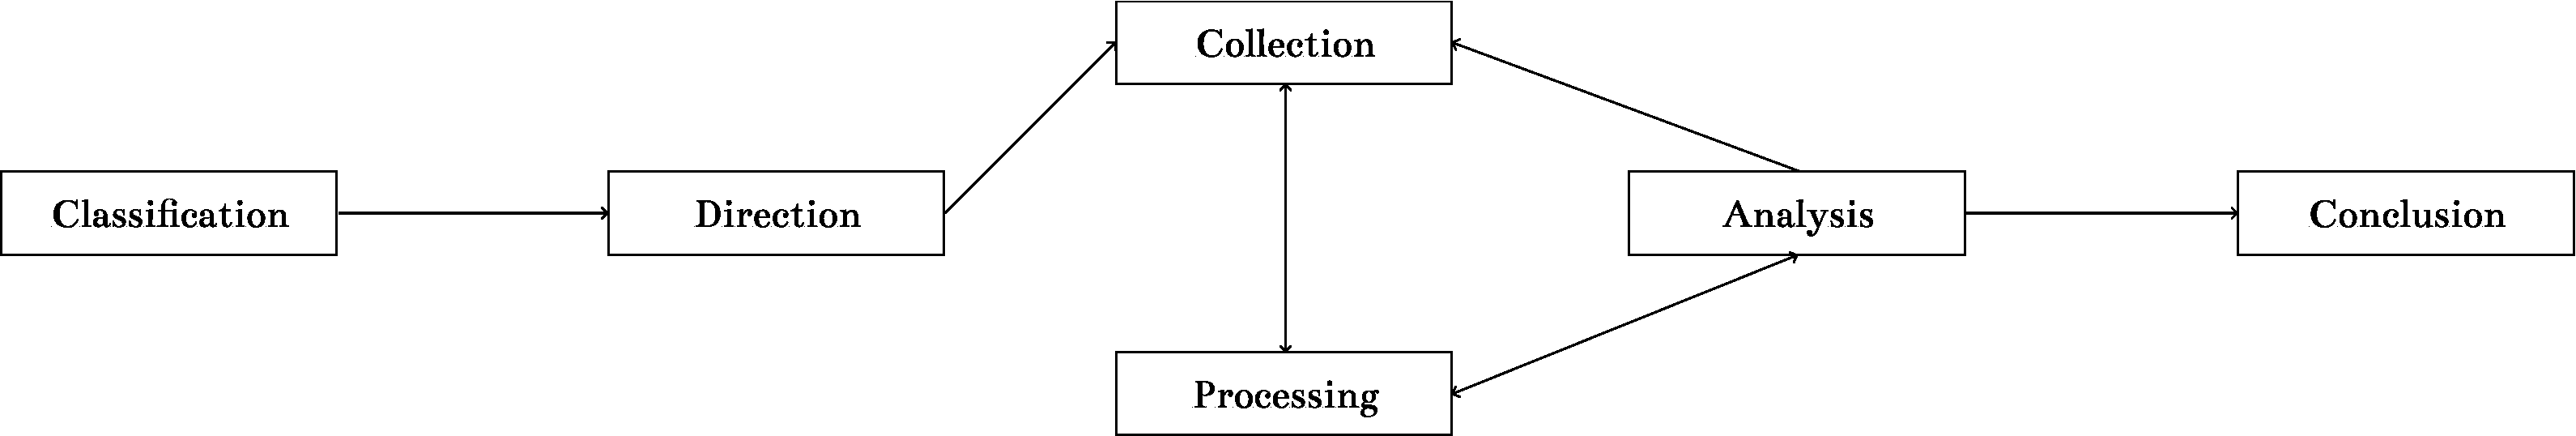
\includegraphics[scale = 0.3]{Model1.pdf} 
    \caption{A Contemporary Intelligence Model}
    \label{A Contemporary Intelligence Model}
\end{figure}

This figure uses most of the same terms and classifications as the original intelligence model, but changes the nature of the model drastically in two ways. First, the model is no longer purely linear, it incorporates elements which can occur simultaneously. Second, the model has feedback loops, as indicated through the use of bi-directional arrows. \\

The process begins with classification. The actions taken at each step of this intelligence cycle are slightly different for each type of intelligence operation. For example, collection in a covert operation would look different than collection in a counterintelligence operation. For this reason, it is important that intelligence begin by classifying a particular project into a category. \\

Following classification, each project needs direction, which includes planning and proper resource allocation. This aspect is very similar to the direction and planning phase of the traditional intelligence cycle. It seems intuitive to place this linearly following classification of the project, as it is not possible to do much without first devising a plan and having the resources needed to continue a mission or project. \\

Following direction, collection begins. While collection of information is critical for any type of operation, it is more nuanced than one might first imagine. Because collection need not be completed for processing to being, collection is placed parallel to processing, implying that the two occur simultaneously to some extent. Here, the first bi-directional arrow of the model is seen. This bi-directional arrow exists because while collection of data is certainly required to process it, processing data may show a need to collect more data or a different type of data. Thus, information flows back and forth between the collection and processing stage often, as the individuals following this model keep refining their collection and processing for information that will yield the most fruit. \\

Following collection, the second bi-directional arrow can be seen between processing and analysis. While the traditional intelligence model finds that the relationship between processing and analysis is linear, the new model implies that this is not the case. Instead, steps taken during the analysis process may demonstrate a need for more processing to be done. This processing, in turn, may require more collection, leading us to the relationship between processing and collection explained above. \\

Analysis of processed information may also lead to the conclusion that fundamentally irrelevant information was collected originally, leading the analysis to cause more collection. Importantly, this arrow is not bi-directional. For intelligence to be used in an analysis, it must be processed for the analyst to make sense of it. For this reason, moving from the analysis stage back to the collection stage requires that collection lead to processing, then analysis again. \\

After this analysis has been completed, there exists some sort of conclusion. This term is intentionally left vague due to the variety of ways a project can conclude. Of course, most traditional intelligence projects may end with dissemination, as the current intelligence cycle suggests. In cases of covert action or counter-intelligence, though, this conclusion may present itself as concrete action or policy-implementation. Regardless, this step indicates any final action taken on a project and implies completion of the project's original goal.

\subsection{Covert Action \& Counterintelligence}
This model also addresses covert action and counterintelligence. While the classification, direction, and conclusion states are all the same for covert action and counterintelligence, the collection, processing and analysis sections differ slightly. \\

For counterintelligence, the direction phase is equivalent to penetrating any necessary system, as this penetration can be thought of as ascertaining a resource necessary for intelligence collection. The analysis phase would then become equivalent to interdiction, wherein a decision is made between pre-empting an action or arresting the violators. \\

For covert action, the only significant difference would be in analysis, which would use information option creation. If no viable options were created, more processing or collection could occur with the model until enough options were created for a viable option to be selected amongst them, with the conclusion consisting of option selection. \\

A model more clearly depicting these differences can be seen below. \\

\begin{figure} [h!]
    \centering
    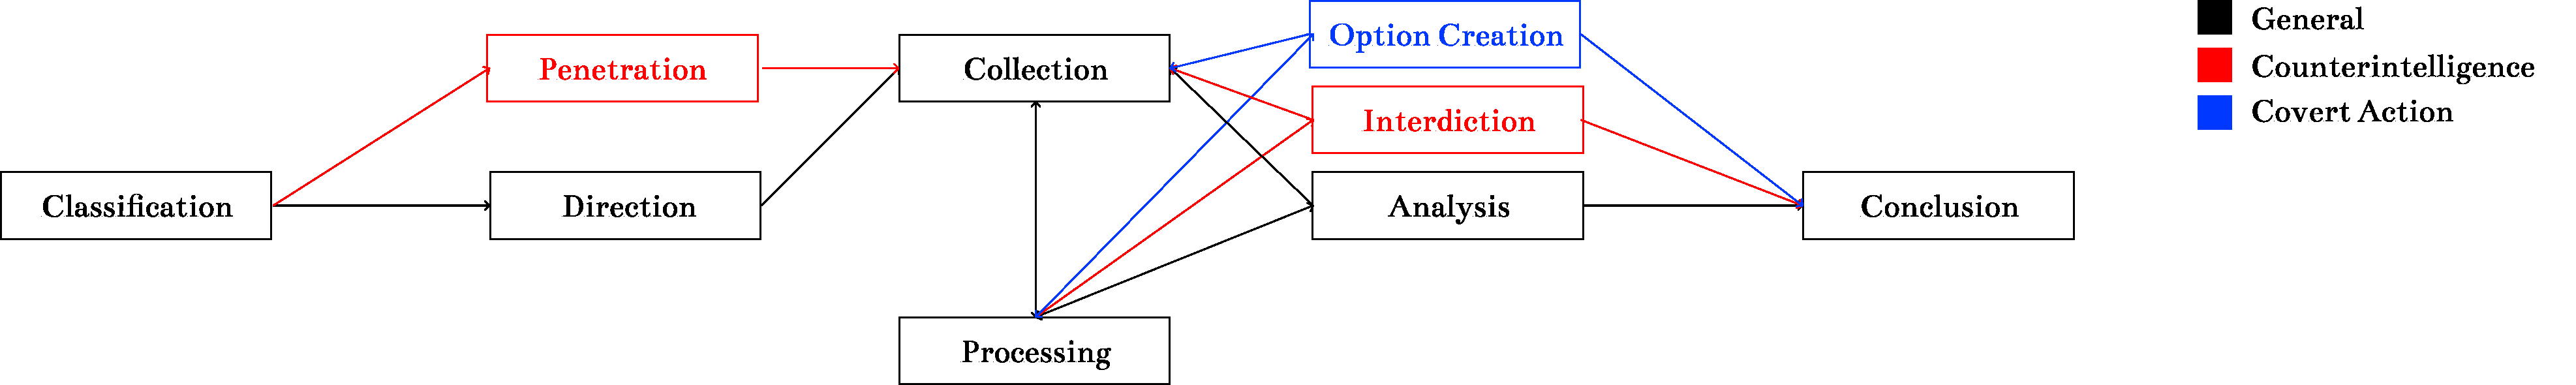
\includegraphics[scale = 0.25]{Model2.pdf} 
    \caption{Illustrating the Role of Covert Action \& Counterintelligence}
    \label{Not Your Father's Intelligence Model}
\end{figure}

Of course, this model is significantly harder to follow. This paper accordingly suggests simply using the original model, replacing definitions as necessary based on classification.

\subsection{Solvency}
Indeed, this model solves each problem with the current intelligence cycle. The model is no longer linear and discrete. Rather, it incorporates both simultaneity and feedback. Secondly, this intelligence model is no longer predicated upon the cognitive decision-making process. It acts as a consolidated unit. Any problem that occurs in one phase of the process can be corrected by following the cycle (eg. reverting back to collection when analysis discovers there is insufficient information to make a conclusion.) Third, this cycle can handle explaining counter-intelligence and covert operations much more elegantly, as explained in the previous section. Finally, this model is much more modern, as seen through the simultaneous nature of collection and processing. Because modern software has the ability to process much information soon after, if not at the same time as collection, these two steps occur in tandem.

\newpage
\section{Conclusion}
This paper does not argue that the model here is the best one possible, nor does it capture an amalgam of operation scenarios. It is, however, a more realistic model than the intelligence cycle used today, while still retaining the intuitive and elegant nature that makes the current intelligence cycle so appealing.

In its attempt to retain this intuitive, elegant nature, this model does not address many outside influences that may occur at stages along the intelligence cycle, nor is it as cohesive as the author would like when discussing covert action specifically. Addressing these shortcomings, however, would have made the model more complicated than it should be. Because this model has virtue only insofar as it can be easily understood by those learning about strategic intelligence, adding more to it for the sake of realism would have been counterproductive.

\newpage
\section{Works Cited}
\begin{enumerate}
    \item Hulnick, Arthur. 2015. "What's Wrong with the Intelligence Cycle?" In \textit{Essentials of Strategic Intelligence}. Johnson, Loch K. pp 67-91. ISBN 1440832285.
    
    \item  Johnson, Loch. 2003. "Bricks and Mortar for a Theory of Intelligence". Comparative Strategy. 22:1. 1-28. DOI: 10.1080/0149593039013048
    
    \item  Philip Davies, Kristian Gustafson, Ian Rigden. 2013. "The intelligence cycle is dead, long live the intelligence cycle: Rethinking intelligence fundamentals for a new intelligence doctrine." \\ http://bura.brunel.ac.uk/handle/2438/11901 
    
    \item Warner, Michael. 2013. "The past and future of the Intelligence Cycle." In \textit{Understanding the Intelligence Cycle}. Phythian, Mark. pp 9-19. ISBN 9780203558478.
\end{enumerate}
\end{document}